\documentclass[handout]{beamer}

\usepackage{fontspec} 
% \usepackage{lsp-makros}
\useoutertheme{lsp}

\usepackage{lsptitle}
\usepackage[german]{babel}

\def\two@digits#1{\ifnum#1<10 0\fi\number#1}
\def\mytoday{\two@digits{\number\day}.\two@digits{\number\month}.\number\year}


\usepackage{xspace,multicol}
\newcommand{\latex}{\LaTeX\xspace}
\usepackage{tikz}


\newcounter{lastpagemainpart}
\footnotesep0pt
\renewcommand{\footnoterule}{}
\usefootnotetemplate{
  \noindent
  \insertfootnotemark\insertfootnotetext}

\let\beamerfn=\footnote
\renewcommand{\footnote}[1]{%
\let\oldfnsize=\footnotesize%
\let\footnotesize=\tiny%
\beamerfn<\thebeamerpauses->{#1}%
\let\footnotesize=\oldfnsize}


\date{\today}

\usepackage{eurosym}  
 
\renewcommand{\centerline}[1]{\hfill#1\hfill\hfill\mbox{}}


\title{Open Access in der\\ Sprachwissenschaft\medskip\\\Large Eine Disziplin stellt um.}
% \institute{FU Berlin}
\author[Nordhoff]{Sebastian Nordhoff}



\begin{document}
\lspbeamertitle


\frame{
\frametitle{Überblick}
%   \includegraphics[height=.2\textheight]{./path/to/graphicsfile}
  \tableofcontents
}
 
\section{Linguistik}
 \frame{
\frametitle{Linguistik}
%   \includegraphics[height=.2\textheight]{./path/to/graphicsfile}
  \begin{itemize}
       \item    25\,000 Linguisten weltweit
       \item        Abgrenzungsprobleme
       \begin{itemize}
       \item            Philologien
       \item            Sprachpädagogik
       \end{itemize}
       \item        ungefähr genau so viele wie Teilchenphysiker
       \item    \glqq die naturwissenschaftlichtste unter den Geisteswissenschaften\grqq
       \begin{itemize}
         \item Publikationssprache englisch
         \item Artikel \& Bücher
         \item Peer Review etabliertes Verfahren
       \end{itemize}
  \end{itemize}
}

\frame{
\frametitle{Sebastian Nordhoff}
%   \includegraphics[height=.2\textheight]{./path/to/graphicsfile}
  \begin{itemize}
    \item          Linguist
    \begin{itemize}
      \item Sprachen Paraguays und Sri Lankas
    \end{itemize}
       \item    Entwickler
       \begin{itemize}
       \item        Glottolog-Datenbank mit 300.000 bibliographischen Referenzen und 27.000 Sprachen, Dialekten und Sprachfamilien
       \end{itemize}
       \item    Open Everything activist
       \item    Geschäftsführer von Language Science Press
       \item    Mitarbeiter im Projekt KOALA bei der TIB
  \end{itemize}
  
\includegraphics[height=1.5cm]{koala.jpg}
  
\includegraphics[height=1.5cm]{tib.jpg}
  
\includegraphics[height=1.5cm]{langsci_logo_nocolor}
}



\section[OA in der Linguistik]{Open Access in der Sprachwissenschaft}
\frame{
\frametitle{Open Access in der\\ Sprachwissenschaft}
  \bigskip
\includegraphics[height=.3\textheight]{glossa.png}\\~\\

  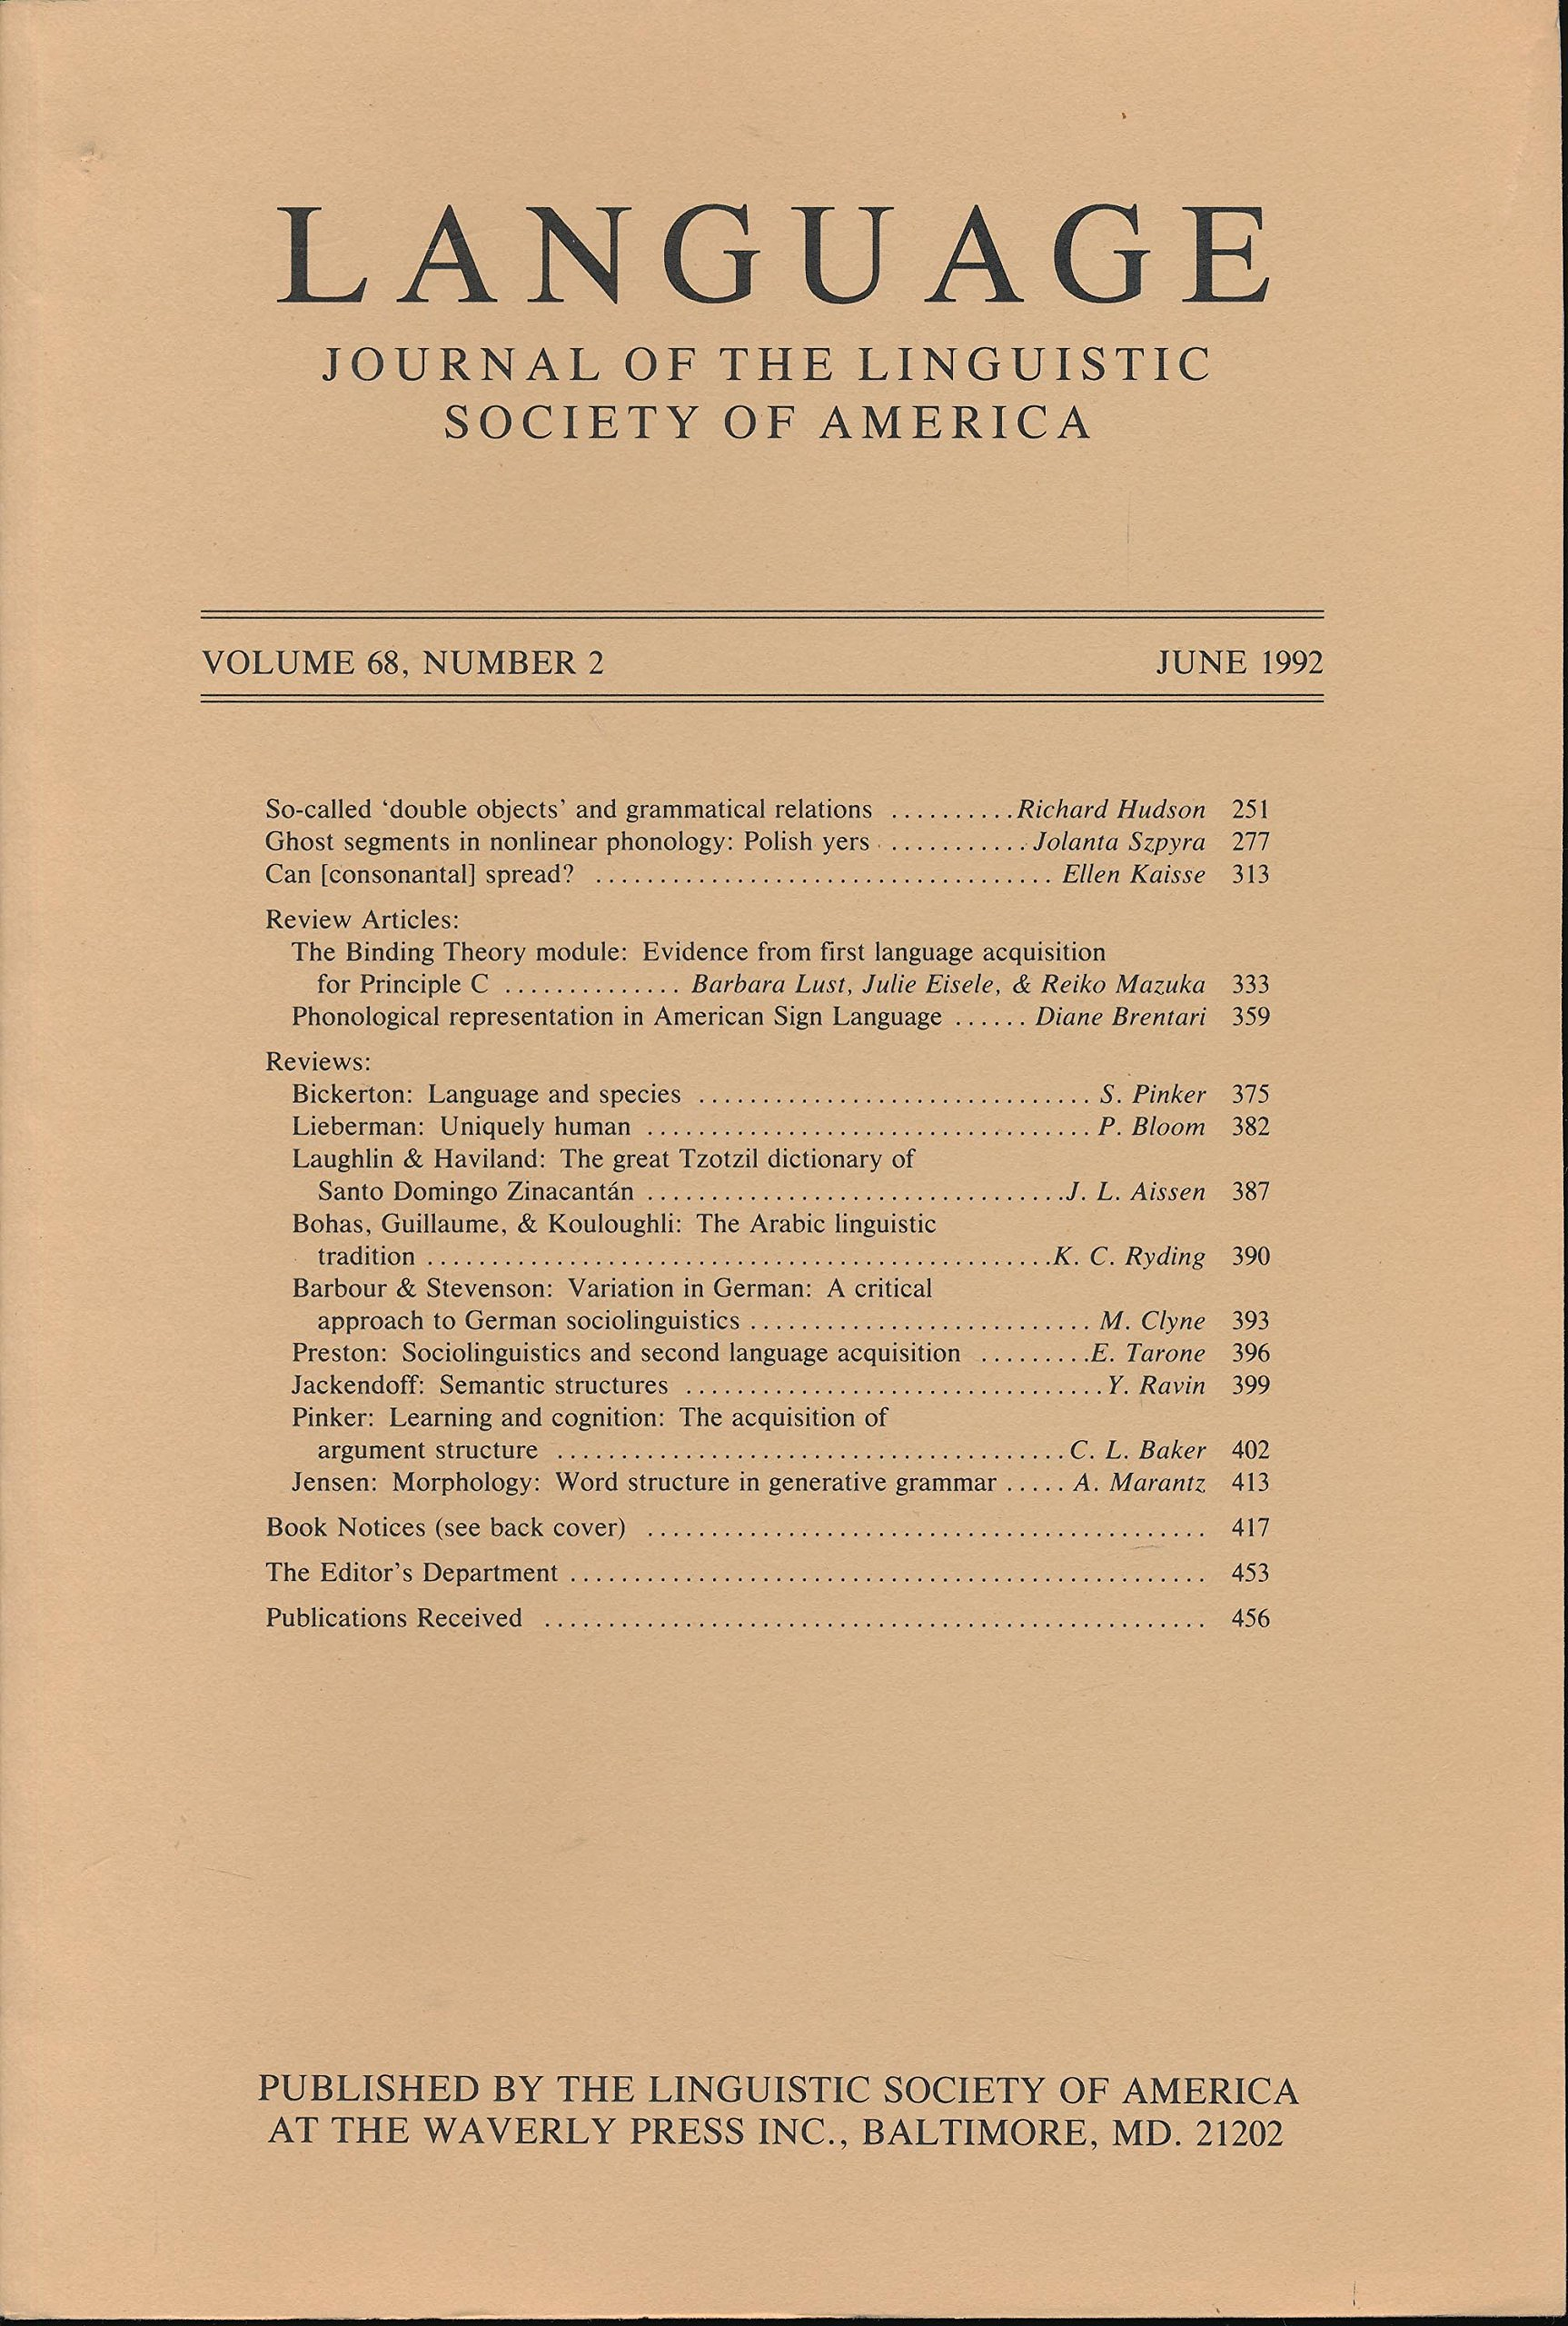
\includegraphics[height=.4\textheight]{language.jpg}
  
\includegraphics[height=.4\textheight]{zfs.jpg}
  
\includegraphics[height=.4\textheight]{langsci_logo_nocolor.pdf}

}

\subsection{Lingua/Glossa}
\frame{
\frametitle{Lingua/Glossa}
%   \includegraphics[height=.2\textheight]{./path/to/graphicsfile}
  \begin{itemize}
    \item  Gegründet 1949
    \item gehört Elsevier
    \item Hybrid-Zeitschrift mit APCs von derzeit USD 2\,890
    \item Die Herausgeber traten 2015 in Verhandlungen mit Elsevier, um \textbf{Fair Open Access} zu erreichen. Dazu gehörten u.a. transparente und vertretbare Autorengebühren
    \item Elsevier war zu keinen Zugeständnissen bereit
    \item Konsequenz: alle Herausgeber und das gesamte Editorial Board traten zurück und gründeten \textit{Glossa}

%        \item       \url{https://www.insidehighered.com/news/2015/11/02/editors-and-editorial-board-quit-top-linguistics-journal-protest-subscription-fees}
%        \item       \url{https://www.heise.de/tp/news/Elsevier-Abtruennige-gruenden-neues-Open-Access-Journal-2912220.html}
%        \item       \url{https://www.wired.com/2015/11/editors-of-the-journal-lingua-protest-quit-in-battle-for-open-access}
%        https://languagelog.ldc.upenn.edu/nll/?p=34106

  \end{itemize}
}



\frame{
\frametitle{Lingua/Glossa heute}
%   \includegraphics[height=.2\textheight]{./path/to/graphicsfile}
  \begin{itemize}
    \item           Glossa
        \begin{itemize}
                \item          2016--2021 = 5,5 Jahre
                \item          700 Artikel
                \item              120 Artikel/Jahr
                \item          im großen und ganzen gleiche Autorenschaft wie vorher
        \end{itemize}
    \item      Zombie Lingua
        \begin{itemize}
        \item           2020: 102 Artikel
%         \item                  <https://www.sciencedirect.com/journal/lingua/vol/168/suppl/C>
%         \item                      <https://www.sciencedirect.com/journal/lingua/vol/244/suppl/C>
        \item          andere Autorenschaft
            \begin{itemize}
            \item              Ostasien
            \item              Arabische Welt
            \item              Iran
            \end{itemize}
        \end{itemize}
  \end{itemize}
}

\frame{
\frametitle{Lingua 170 (2016) vs.\\ Lingua 258 (2021)}
\hfill
  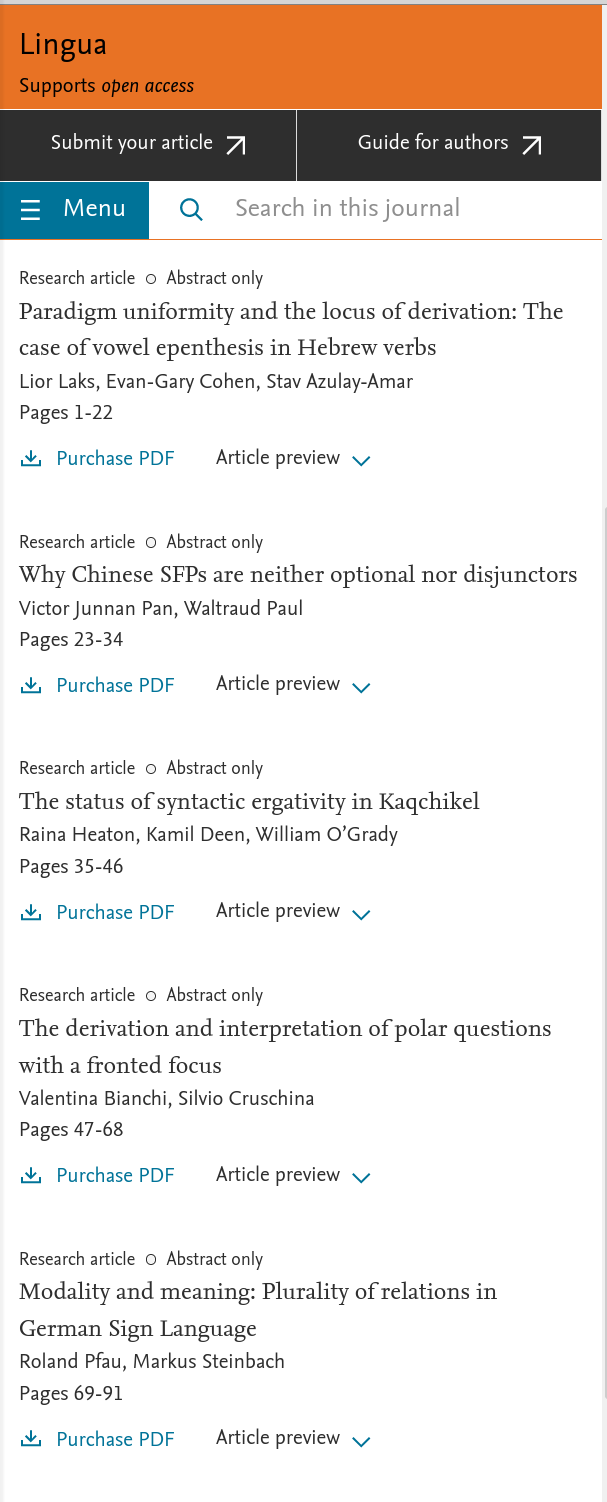
\includegraphics[height=\textheight]{lingua-alt.png}
  \hfill
  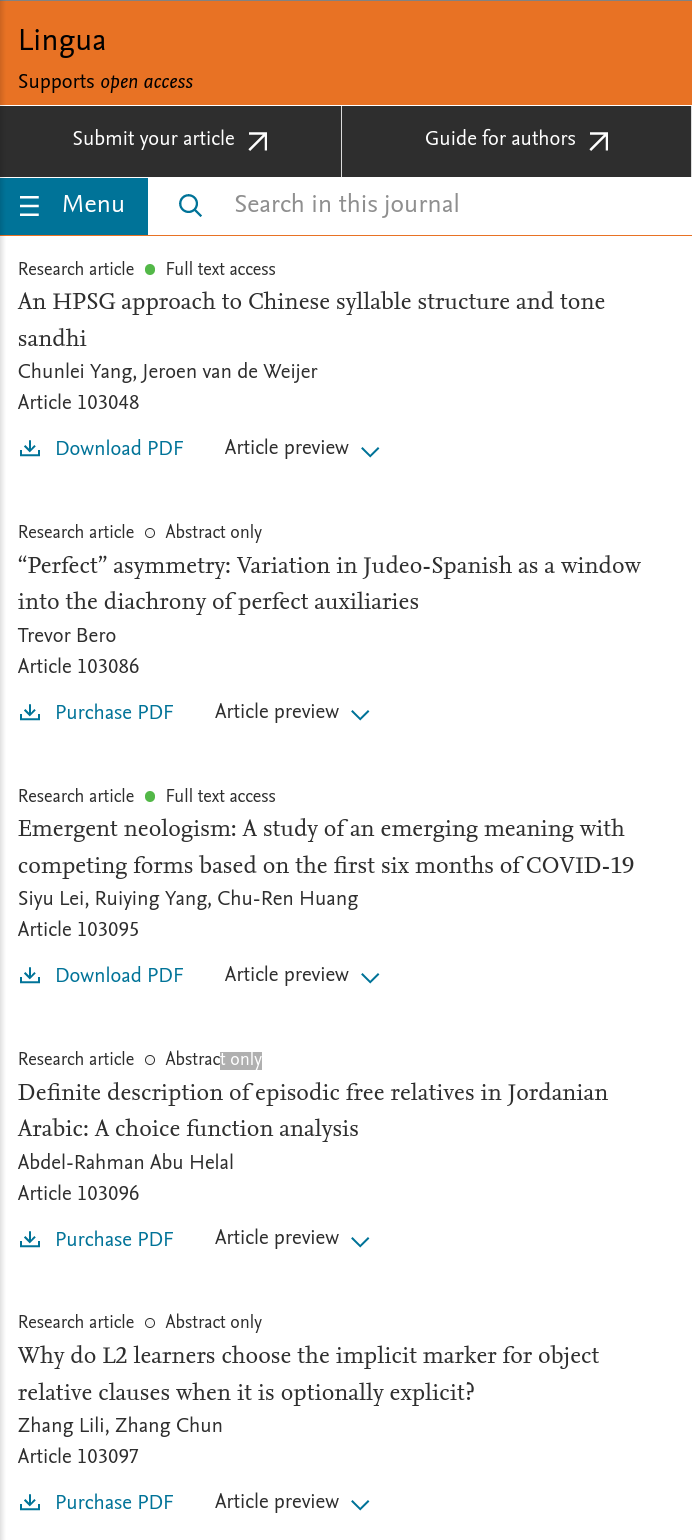
\includegraphics[height=\textheight]{lingua-neu.png}
  \hfill~
}


 \frame{
\frametitle{LingOA}
%   \includegraphics[height=.2\textheight]{./path/to/graphicsfile}
{\small
LingOA will provide a framework for the smooth transition from the traditional journal subscription model to Fair Open Access publishing. LingOA aims at developing an affordable and sustainable business model for Open Access publishing.

Several leading, international linguistics journals are being transferred from their current traditional publisher to a new Open Access publisher. This open access publisher complies with the following conditions:
}

\begin{enumerate}
  \item  The editorial board owns the title of the journals.
  \item  The author owns the copyright of his articles, and a CC-BY license applies.
  \item  All articles are published in Full Open Access (no subscriptions, no ‘double dipping’).
  \item  Article processing charges (APCs) are low (around 400 euros),  transparent, and in proportion to the work carried out by the publisher.
\end{enumerate}


}

\frame{
\frametitle{LingOA}
\begin{columns}
  \column{5cm}

  \begin{itemize}
        \item Glossa
       \item        Laboratory Phonology
       \item        Journal of Portuguese Linguistics
       \item        Italian Journal of Linguistics
  \end{itemize}
  \column{5cm}\centering
  
\includegraphics[width=4cm]{rooryck.png}\\Johan Rooryck\\Former editor of \textit{Lingua}\\Editor of \textit{Glossa}\\\mbox{Executive director cOAlition S}
  \end{columns}
}


\subsection{Zeitschrift \glqq Language\grqq}
\frame{
\frametitle{Zeitschrift \glqq Language\grqq}
\begin{columns}
  \column{6cm}
  \begin{itemize}
       \item    Referenz-Zeitschrift in der Linguistik
       \begin{itemize}
         \item man freut sich sehr, wenn dort ein Artikel akzeptiert wird
       \end{itemize}
       \item    gehört der \textit{Linguistic Society of America}
       \item    12 Monate Embargo, danach freier Zugriff
       \item seit 2013 verbleibt das Copyright bei den Autorinnen.
%        \pause
%        \item    mentimeter
%        \pause
%        \item    400 EUR APCs
  \end{itemize}
  \column{4cm}
  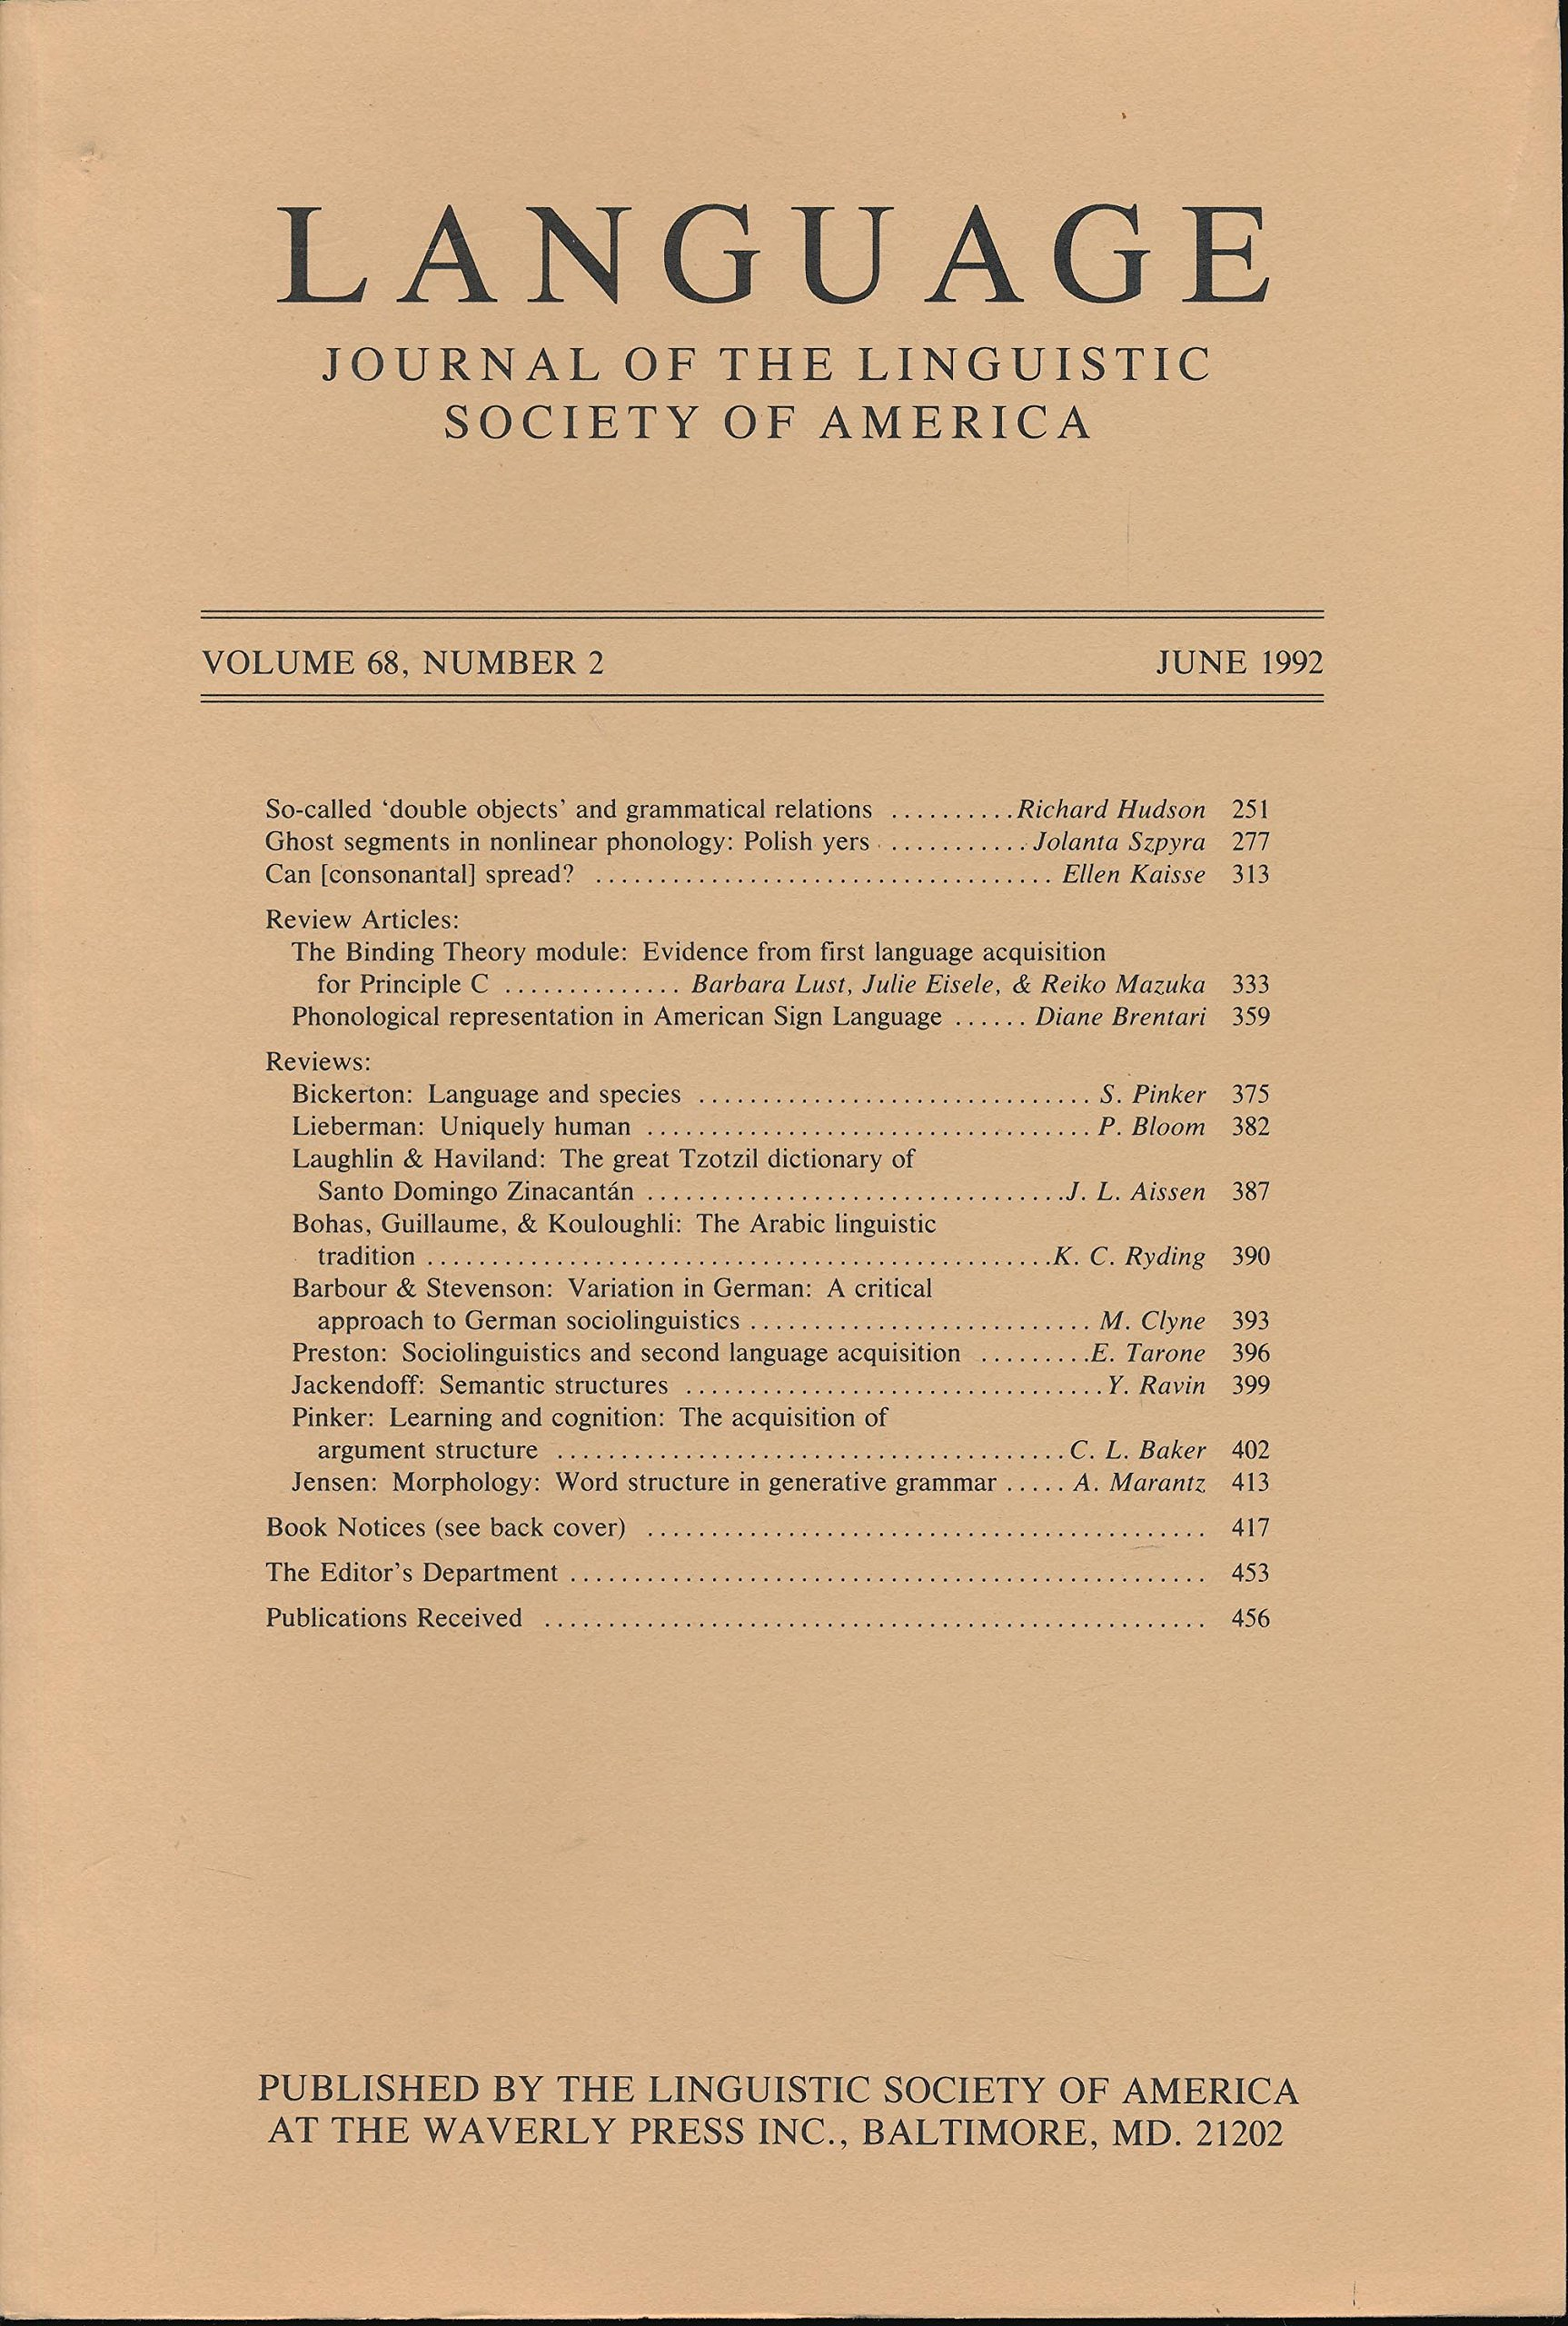
\includegraphics[width=3cm]{language.jpg}
\end{columns}
}


\subsection{Zeitschrift für Sprachwissenschaft}
\frame{
\frametitle{Zeitschrift für\\ Sprachwissenschaft}
%   \includegraphics[height=.2\textheight]{./path/to/graphicsfile}
  \begin{itemize}
     \item    Zeitschrift der \textit{Deutschen Gesellschaft für Sprachwissenschaft}
     \item    historisch hybrid mit APCs
     \item    Umstellung
     \begin{itemize}
     \item        2012 erste Wünsche aus der Mitgliederschaft
     \item    Druck auf folgenden DGfS-Jahrestagungen
     \item    2015 Umstellung auf \glqq Learned Society Pays\grqq
     \end{itemize}

  \end{itemize}
}

\frame{
\frametitle{Zeitschrift für\\ Sprachwissenschaft}
%   \includegraphics[height=.2\textheight]{./path/to/graphicsfile}
  \begin{itemize}
    \item         DGfS übernimmt APCs in Höhe von 1200 EUR
    \begin{itemize}
      \item         800 EUR sind die Kosten von de Gruyter, gut informierten Kreisen zufolge
       \item        400 EUR wären möglich
       \item        Immer noch besser als 2000 EUR wie im naturwissenschaftlichen Bereich oder 2890 USD wie bei Lingua
    \end{itemize}
       \item    Autorinnen behalten Copyright
       \item    Gesellschaft hatte nachher mehr Geld als vorher
       \begin{itemize}
            \item  Stiftung eines OA-Preises
       \end{itemize}
       \item anekdotisch: mehr Einreichungen
  \end{itemize}
}


\subsection[LangSci Press]{Language Science Press}
\frame{
\frametitle{Language Science Press}
%   \includegraphics[height=.2\textheight]{./path/to/graphicsfile}
  \begin{itemize}
      \item     OA-Bücher
      \begin{itemize}
        \item         Monographien
        \item         Sammelbände
      \end{itemize}
      \item     Idee 2012 (Martin Haspelmath, Stefan Müller)
      \begin{itemize}
        \item Hintergrund: De Gruyter ``depublizierte'' Stefan Müllers Buch
      \end{itemize}
      \item     DFG-Projekt 2014-2016
      \item     Humboldt-Universität zu Berlin 2017-2018
      \item     Seit 2018 konsortial finanziert über Knowledge Unlatched
  \end{itemize}
}
\frame{
\frametitle{Language Science Press}
%   \includegraphics[height=.2\textheight]{./path/to/graphicsfile}
  \begin{itemize}
    \item         Autorinnen behalten Copyright
       \item   170 veröffentlichte Bücher
       \begin{itemize}
            \item   60-1600 Seiten
       \end{itemize}
       \item 30 Bücher im Jahr
       \item Kosten: 120\,000€ im Jahr
       \begin{itemize}
                \item $\to$ kalkulatorisch 4\,000 €/Buch
       \end{itemize}

       \item   Diamond OA
       \item   keine Autorengebühren
  \end{itemize}
}

\frame{
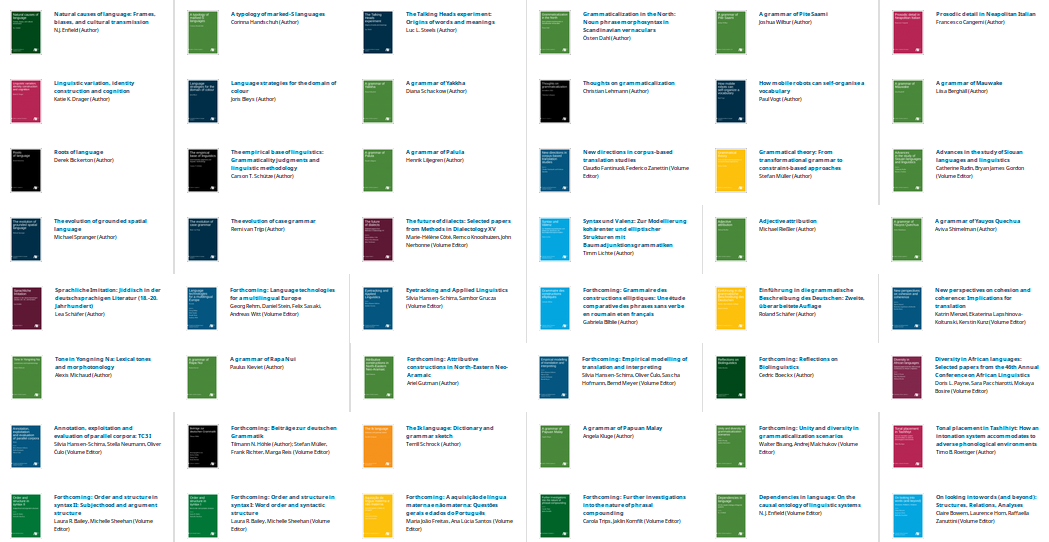
\includegraphics[height=\textheight]{catalog.png}
}

\section{Warum die\\ Sprachwissenschaft?}
\frame{
\frametitle{Warum die Sprachwissenschaft?}
%   \includegraphics[height=.2\textheight]{./path/to/graphicsfile}
  \begin{itemize}
     \item      Chomsky
     \item          Chomsky gehört zu den bekanntesten Linguisten der Gegenwart, wurde aber auch als Kapitalismus- und Globalisierungskritiker weltweit bekannt.
     \end{itemize}
     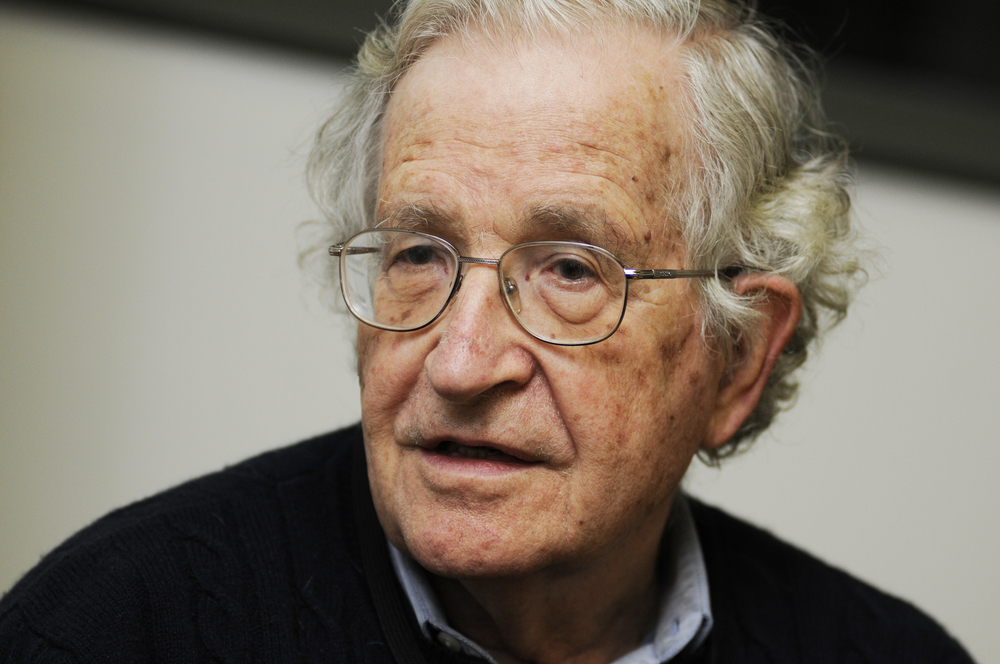
\includegraphics[width=4cm]{chomsky.png}
     }


\frame{
\frametitle{Warum die Sprachwissenschaft? Feldforscher}
\begin{columns}
\column{8cm}
     \begin{itemize}
     \item Marian Klamer
        \begin{itemize}
        \item \textit{The Alor-Pantar languages}, eins der ersten Bücher bei Language Science Press kam von einem anderen Verlag, da die Herausgeberin wollte, das auch Menschen in Indonesien Zugriff auf das Buch haben können.
            \begin{itemize}
            \item Stand heute: 30\ 000 Downloads
            \end{itemize}
            \end{itemize}
     \item  Larry    Hyman
        \begin{itemize}
            \item 7 Kapitel in 5 LangSci-Büchern, Präsident der Linguistic Society of America)
            \item          I join my many colleagues who seek to produce open-access publications whenever possible.
            \item          Open-access is thus a logical extension of how we have always operated. Is it not like this in other fields?
            \end{itemize}
    \end{itemize}

\column{2cm}
     
\includegraphics[height=3cm]{klamer.jpg}
     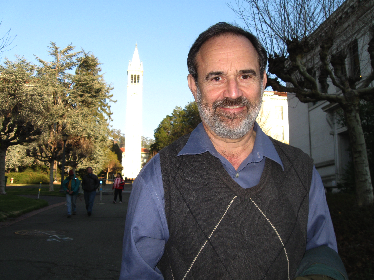
\includegraphics[height=2cm]{larryhyman.png}
\end{columns}
}


\frame{
\frametitle{Warum die\\ Sprachwissenschaft?}

     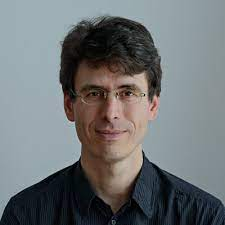
\includegraphics[height=3cm]{stefanmueller.jpg}
     \includegraphics[height=3cm]{martinhaspelmath.jpg}

     \begin{itemize}
       \item Überzeugungstäter mit Nervpotential
       \item jeweils großes internationales Netzwerk
       \item erklären den Forscher*innen gerne, warum das so nicht geht und warum das anders muss und wie das anders gehen kann
       \item gerne auch mehrmals und auch denen, die es nicht hören wollen
       \item Steter Tropfen höhlt den Stein
     \end{itemize}

}


\frame{
\frametitle{Verlagslandschaft}
%   \includegraphics[height=.2\textheight]{./path/to/graphicsfile}
  \begin{itemize}
    \item  Dick Fisher: Die Linguistik hat eine sehr spezielle Verlagslandschaft
    \item recht wenige Verlage, klein bis mittelgroß
    \item keine amerikanischen Universitätsverlage
    \item insgesamt eine sehr übersichtliche Landschaft.
    \item Cambridge University Press, Oxford University Press, de Gruyter, John Benjamins
    \begin{itemize}
      \item Narr, Harrassowitz, Lincom, Routledge, Brill
    \end{itemize}
    \item Parallelen zur Teilchenphysik und SCOAP3?
  \end{itemize}
}

\section{Community-based Publishing}
\frame{
\frametitle{Community-based Publishing\\disziplinäre Netzwerke}
%   \includegraphics[height=.2\textheight]{./path/to/graphicsfile}
  \begin{itemize}
       \item   Scholar-led statt stakeholder-led
       \item    Netzwerke
       \begin{itemize}
       \item        disziplinäre Netzwerke
       \item Forscher*innen mit Fachbezug
       \item Fachbezug stabil
       \end{itemize}
       \item            Name Recognition
            \begin{itemize}
                \item Ah, der ABC Verlag. Da hat doch die XYZ veröffentlicht!
            \end{itemize}
       \item            Prestige
            \begin{itemize}
                \item Ich veröffentliche da, wo die Koryphäen meines Fachs veröffentlichen, dann werde ich bestimmt auch eine Koryphäe
            \end{itemize}
       \end{itemize}
       }

\frame{
\frametitle{Community-based Publishing\\regionale Netzwerke}
       \begin{itemize}
         \item Universitätsverlage
         \item Forscher*innen mit geographischem Bezug
         \item geographischer Bezug häufig temporär
         \item geringe Name Recognition von Forscher*innen im gleichen geographischen Bereich.
         \begin{itemize}
           \item Dr. Schmitz publiziert auch bei Neustadt University Press? Nie gehört! Wer soll das sein?
           \item Selbst wenn Dr. Schmitz den Nobelpreis gewonnen haben sollte, wird das Prestige nicht auf Forscher*innen in anderen Disziplinen abfärben
         \end{itemize}
       \end{itemize}
}


%\setcounter{framenumber}{\thelastpagemainpart}
\end{document}
